\documentclass[16pts]{report}
\usepackage[utf8]{inputenc}
\usepackage[T1]{fontenc}
\usepackage[francais]{babel}
\usepackage{xcolor}
\usepackage[hyphens]{url}
\usepackage[hidelinks]{hyperref}
\usepackage{amsmath}
\usepackage{graphicx}
\usepackage{geometry}
\usepackage{textcomp}
\hypersetup{hypertexnames=true}
\geometry{hmargin=2.5cm,vmargin=1.5cm}

%\maketitle
%\clearpage

\begin{document}
\bibliographystyle{unsrt}
\nocite{*}

\chapter{Contexte}
Il est possible de compiler soi-même un noyau Linux. Cela permet de créer
    un noyau répondant uniquement aux besoins de l’utilisateur. La tâche peut
    être très fastidieuse car les outils permettant de modifier le fichier
    de configuration ne sont pas simples d’utilisation et il est difficile
    de trouver les options que l’on aimerait avoir.

Ce projet a pour but de proposer un outil permettant à un utilisateur non expert
    de configurer simplement son noyau en l'allégeant à sa guise.

\chapter{Configuration des options du noyau}
La principale tâche à effectuer avant de lancer la compilation du noyau est
    de créer un fichier “.config” comportant toutes les options disponibles
    pour le noyau.  Après avoir récupéré le noyau (sur Kernel.org) on constate
    qu’il n’y a pas de fichier “.config” par défaut. Il faut donc le générer et
    plusieurs options s’offrent à nous :

Récupérer le fichier “.config” d’un noyau sur l’ordinateur que l’on souhaite,
    mais il risque d’y avoir des incompatibilités à cause de la version
    des noyaux.

\begin{description}
    \item[make oldconfig :] Qui permet de récupérer la configuration du noyau
        courant et corrige le problème précédent car en cas d’options
        différentes, le système demandera à l’utilisateur de choisir. Il sera
        difficile d’optimiser ce fichier dans le cas où le noyau courant
        contient des options inutiles.

    \item[make defconfig :] Qui permet de générer un fichier de configuration
        minimale.  C’est la meilleure option permettant d’optimiser son noyau
        sans repartir de zéro.  Malgré tout, il crée une configuration
        "minimale" générique et non adaptée à la machine de l’utilisateur.
        Le fichier peut donc être optimisé.
\end{description}

Après avoir généré une configuration initiale, il est possible d’utiliser
différents outils pour la modifier tels que :

\begin{description}
    \item[make config]      	Un programme en ligne de commande \\
        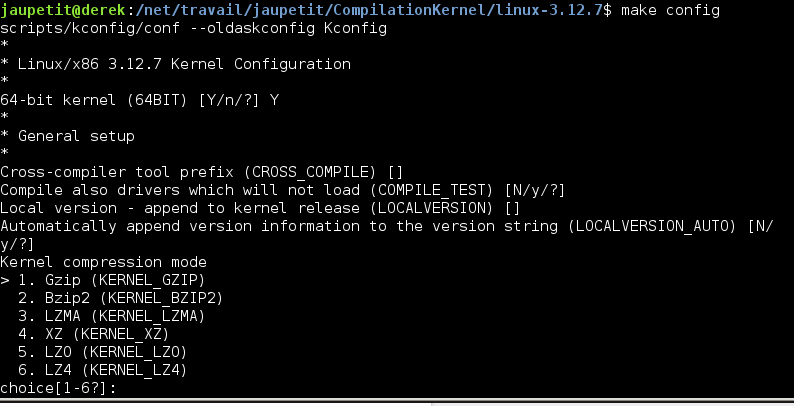
\includegraphics[scale=0.7]{illustrations/configLine.png} \pagebreak
    \item[make menuconfig]      Un programme utilisant ncurse \\
        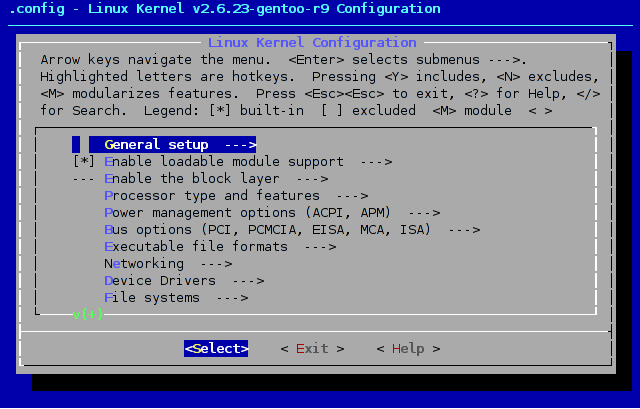
\includegraphics[scale=0.7]{illustrations/menuconfig.png} \\
    \item[make xconfig]     	Un programme utilisant QT \\
        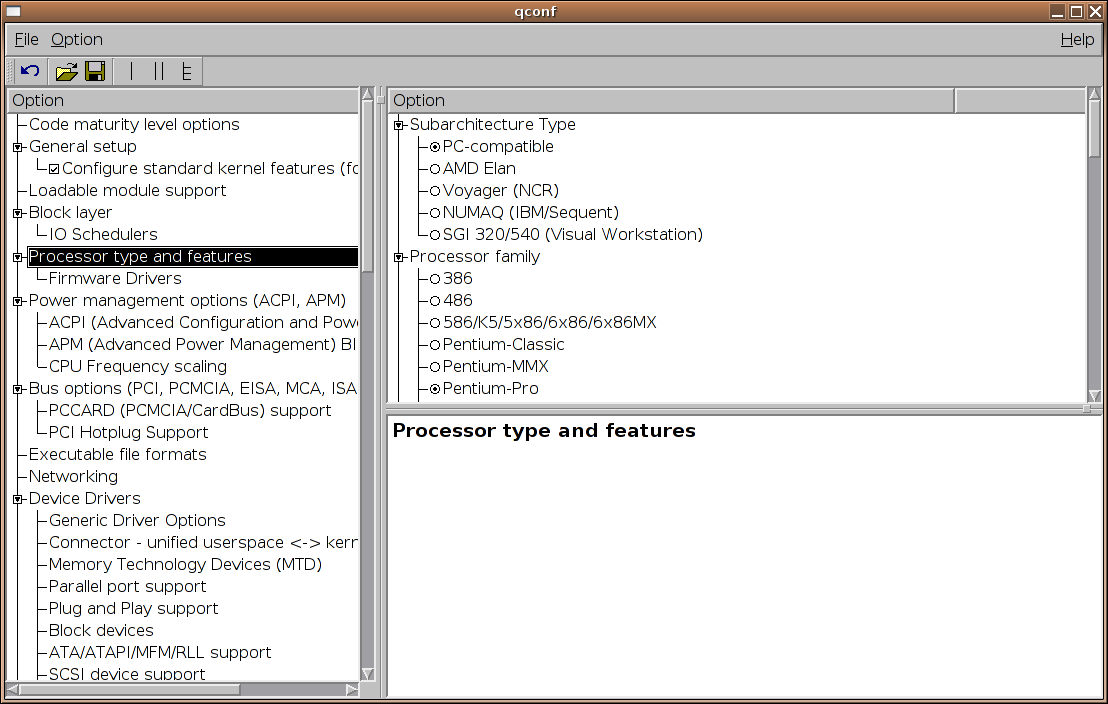
\includegraphics[scale=0.4]{illustrations/xconfig.png} \pagebreak
    \item[make gconfig] 	    Un programme utilisant GTK \\
        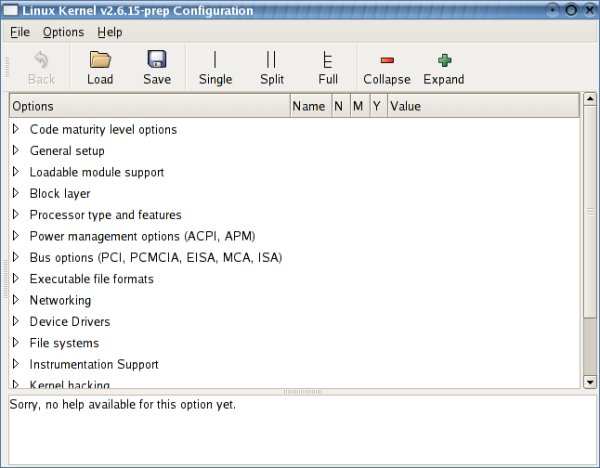
\includegraphics[scale=1]{illustrations/gconfig.jpg} \\
    \item[eCos], qui permet de configurer les noyaux pour le système
        d’exploitation eCos. C’est une autre source d’information
        sur laquelle se baser. \\
        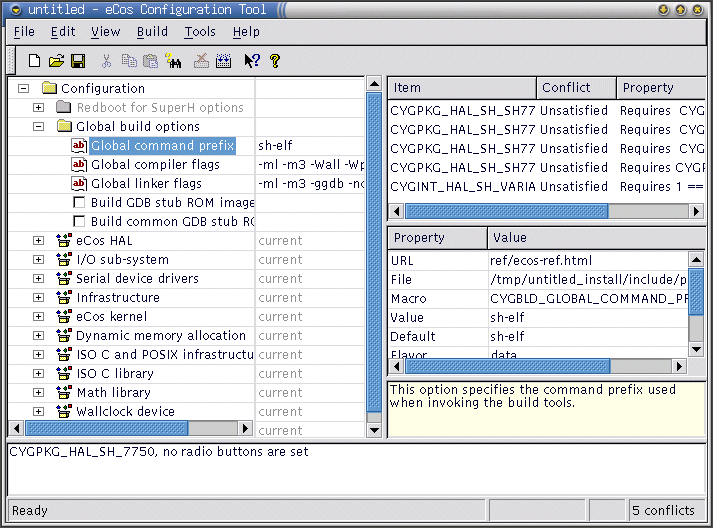
\includegraphics[scale=1.3]{illustrations/eCos_config.png} \pagebreak
    \item[kcheck (kernel check)] permet également de configurer les options d’un noyau
        à compiler.
        Il propose deux modes :

    \begin{description}
        \item[Automatique :] kcheck va tenter de déterminer les options du kernel
            en fonction de la machine sur laquelle il est lancé
        \item[Manuel :] kcheck permet à l’utilisateur de modifier comme bon lui
            semble les différentes options du fichier de configuration du kernel.
    \end{description}
        
\includegraphics[scale=0.8]{illustrations/KernelCheck.png}\\
\end{description}

Une étude a été réalisée par Kacper Bak et Karim Ali de l’université Waterloo
    afin d’améliorer la convivialité de la configuration d’un noyau Linux
    \cite{Waterloo:Etude}.
Celle-ci a permis de mieux cerner les besoins des utilisateurs en observant
    leurs difficultés à utiliser les outils existants. Ils ont réalisé
    un prototype qu’ils ont fait tester et qu’ils ont amélioré afin d’obtenir
    le squelette d’un outil facilitant la configuration d’un noyau Linux. \\

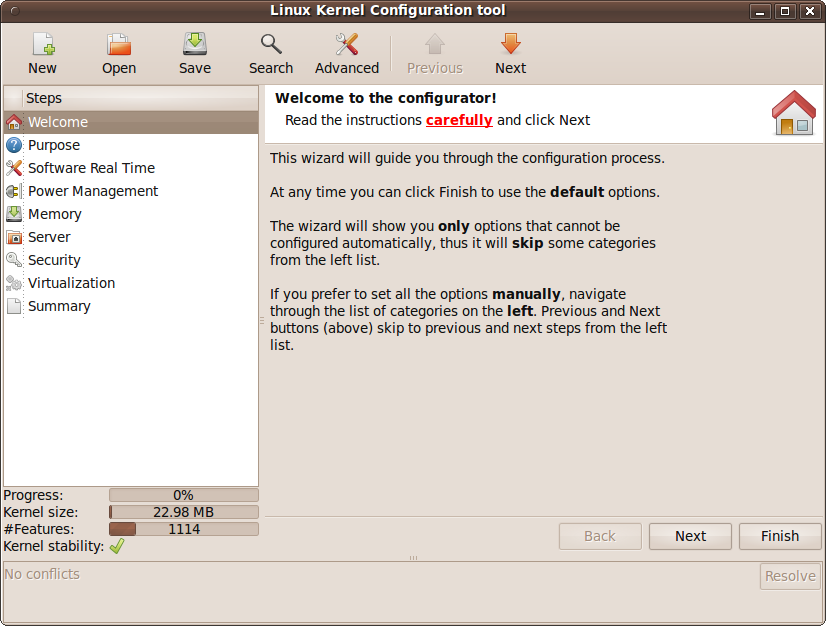
\includegraphics[scale=0.6]{illustrations/lkc-config.png} \\

Leur projet a donc abouti sur un prototype non fonctionnel.
    L’ergonomie de leur application sera une grande source d’inspiration
    pour nous de par les avis qu’ils ont récoltés auprès d’utilisateurs.

Les quatres premiers outils présentés ("config", "menuconfig", "xconfig" et
"gconfig") sont les plus couramment utilisés pour configurer un noyau Linux
avant sa compilation. Nous sommes arrivés à cette conclusion, car dans un
premier temps, ces outils sont présents au sein même des sources du noyau Linux.
Et dans un second temps, en recherchant comment d'autres personnes réalisaient
cette configuration, nous avons constaté qu'ils utilisaient à chaque fois l'un
de ces outils et principalements ceux avec une interface graphique.

Pour ce qui est des deux derniers outils ("eCos", et "kCheck"), ils sont
beacoup moins répandus mais ils répondent à différents besoins de notre projet
dont nous allons nous inspirer :
\begin{itemize}
    \item La gestion des conflits entre les options
    \item La détection du matériel pour générer le fichier de configuration
\end{itemize}

Enfin, le dernier outil est seulement un prototype réalisé par l'université de
Waterloo, mais qui constitue notre plus importante base pour ce projet. En
effet, celui-ci ayant été réalisé après une étude des besoins des utilisateurs,
il comporte des informations précieuses pour réaliser notre PdP.

\chapter{Difficultés de la configuration}

Il existe plusieurs raisons qui font que la configuration des options d’un noyau
    est une tâche fastidieuse et difficile :

Tout d’abord, le principal problème se situe au niveau des conflits et
    des dépendances entre les options. En effet, celles-ci peuvent
    être liées à d’autres options ou même exclusives, c’est à dire que si
    une option est sélectionnée, une autre peut ne plus l’être.
    Le problème de certains des outils actuels est que les options en conflit
    avec les options actuelles ne sont plus visibles. Donc lorsque l’on cherche
    une option précise qui n’est plus affichée et que l’on ne sait pas quelle
    précédente option est en conflit avec elle, il est très difficile de
    corriger cette erreur.

En outre, lorsqu'une option est sélectionnée, les outils actuels désactivent
    automatiquement et sans prévenir l'utilisateur celles qui sont en conflit
    ou celles qui en dépendent.

Enfin, il est compliqué pour un utilisateur non expert de trouver une
    option précise sans la connaître parfaitement. Le nom de cette option
    ne représente pas toujours très bien sa fonction, ce qui fait que
    la recherche des options dans l’outil n’est pas aisée.
    On constate qu’il y a une aide pour chacune des options et
    il est dommage que la recherche par mots-clés ne s’effectue pas également
    sur l’aide des fonctions.

\chapter{Recherches bibliographiques}

Notre sujet se repose sur un projet existant. En effet, l'université de Waterloo
a réalisé une étude approfondie \cite{Waterloo:Etude} sur la facilité
d'utilisation des outils de configuration du noyau Linux. On y trouve les
résultats de leurs tests auprès de différents utilisateurs, ce qui nous permet
d'avoir des informations sur les besoins réels vis à vis de cet outil. L'équipe
a réalisé un prototype qui prend en compte ces modifications et celui-ci peut
être trouvé dans leur dépôt Github \cite{Waterloo:Github}.

Nous avons trouvé d'autres avis d'utilisateurs au sein d'une étude
\cite{Hubaux:2012:USC:2110147.2110164}. On peut y observer les principaux
problèmes qu'ils ont rencontrés. Par exemple, on peut constater que la gestion
des conflits est une fonctionnalité qui pose généralement des difficultés.

Pour mieux comprendre notre sujet, nous avons configuré et compilé un noyau
Linux que nous avons trouvé sur le site officiel \cite{Kernel}. On peut trouver
au sein du dossier téléchargé, différents outils permettant de réaliser la
configuration du noyau avant sa compilation. On y trouve "menuconfig", "xconfig"
et "gconfig" qui sont des outils graphiques plus simple d'utilisation que
l'outil en ligne de commande "config".

La configuration étant difficile, nous avons trouvé sur le forum de Linux
\cite{Existant:Kernel:ForumTutoConfig} des explications très détaillées. Ce
guide reprends "pas à pas" chacune des options et les détaille une à une afin de
mieux comprendre ce qui peut être activé ou non.

Une fonctionnalité qui pourrait être utile pour un utilisateur serait de pouvoir
détecter le matériel de son ordinateur (ou une partie) afin de pouvoir générer
le fichier de configuration correspondant à sa machine. Nous avons trouvé un
tutoriel \cite{Existant:Kernel:outils} traitant de la compilation du noyau Linux
et qui évoque ce point particulier.

Un des problèmes évoqués par les testeurs de l'étude \cite{Waterloo:Etude} de
l'université de Waterloo, est que le système de gestion des conflits des outils
actuels n'est pas pratique, car aucune indication n'est donnée lorsqu'une option
est sélectionnée. Nous avons trouvé un outil qui effectue ce traitement des
conflits, mais pour un système d'exploitation différent : eCos
\cite{Existant:EcosConfig}. En nous en inspirant, nous pourrons éventuellement
proposer un mécanisme similaire dans notre outil de configuration.


L'étude \cite{Waterloo:Etude} explique brièvement comment fonctionne
l'arborescence des modules au sein du noyau Linux. Nous avons donc décidé
d'approfondir ce point et nous avons trouvé un fichier
\cite{Existant:Kconfig:frontends} expliquant plus en détail le fonctionnement
pour l'outil "menuconfig". En reprenant le même mécanisme utilisé par les outils
officiels, nous pourrons éventuellement nous abstenir de refaire le parsage des
nombreux dossiers des sources. Nous avons également récupéré de la documentation
\cite{Existant:Kconfig:vueDensemble} \cite{Existant:Kconfig:langage} qui
contient les éléments de syntaxe qui nous ont aidés à comprendre comment
s'effectue la génération du fichier ".config". De plus, on trouve sur le site
officiel du noyau Linux des indications \cite{Existant:Kconfig:modules}
permettant de compiler un module externe au sein du noyau. Celui-ci nous permet
donc de mieux comprendre le fonctionnement des fichiers "Kbuild".
\bibliography{./bibliographie}
\end{document}
